\chapter{Fahrtage}\label{einsatz:fahrtag}
\section{Allgemeines und Personal}
\begin{figure}[!h]
	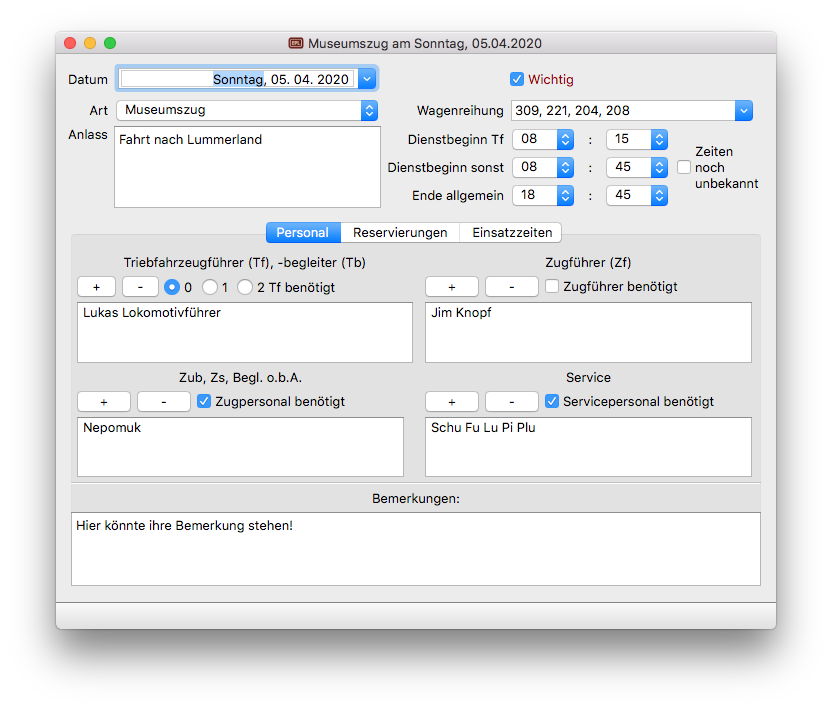
\includegraphics[width=\textwidth]{img/fahrtag_personal}
	\caption{Das Fenster eines Fahrtags mit geöffnetem Tab für das Personal.}
	\label{fig:einsatz:fahrtag:personal}
\end{figure}
\paragraph{Allgemein}
Im oberen Bereich des Fensters können die grundlegenden Daten für einen Fahrtag eingegeben werden.
Dies umfasst zum einen den Tag und die Dienstzeiten.
Sind die Zeiten für den Fahrtag noch unbekannt, können Sie das mit dem entsprechenden Häkchen kenntlich machen.

Ebenso kann die Art und der Anlass der Fahrt angegeben werden.
Die Wagenreihung wirkt sich auf die Anzeige der Reservierungen aus und ist für die Personalplanung wichtig.
Es stehen bereits einige häufige Kombinationen zur Verfügung.
Diese können aber auch beliebig verändert werden.
Dabei müssen die Wagen durch Kommata voneinander getrennt werden.

Eine Markierung als \emph{wichtig} wird beim Export des Fahrtages durch eine optische Hervorhebung gekennzeichnet.
Ebenso kann die Veranstaltung abgesagt werden.
In diesem Fall werden für die eingetragenen Personen keine Stunden angerechnet, sodass diese nicht entfernt werden müssen.
Beim Export werden in diesem Fall nur noch die Rahmendaten und die Bemerkungen ausgegeben.

Darüber hinaus können auch allgemeine Bemerkungen für die Fahrt angegeben werden.


\paragraph{Personal}
In den vier Listen können Tf, Zf, Zub und Begl.o.b.A.\ und Service-Personal eingetragen werden.
Für betriebliche Aufgaben (Tf, Tb, Zf) können nur Personen eingetragen werden, die die entsprechende Ausbildung haben.
(Siehe \cref{personal:person})
Die Namen sind dabei wie folgt einzugeben: \texttt{Name; Bemerkung}.

Da Personal in Ausbildung die entsprechenden Berechtigungen noch nicht hat, können folgende Wörter in der Bemerkung verwendet werden, um diese Personen dennoch in der entsprechenden Liste einzutragen:
\begin{itemize}
	\item Azubi
	\item Ausbildung
	\item Tf-Ausbildung
	\item Zf-Ausbildung
	\item Tf-Unterricht
	\item Zf-Unterricht
	\item Weiterbildung
\end{itemize}
Ein Zugbegleiter ohne Ausbildung wird automatisch als Begl.o.b.A.\ geführt, sodass hier keine Unterscheidung vorgenommen werden muss.

Generell können nur Personen eingetragen werden, die im System bereits registriert wurden und nicht ausgetreten sind
(weiteres im \cref{personal:person,einsatz:personal}).
Auch hier gibt es wieder Ausnahmen, wenn einer der folgenden Begriffe in der Bemerkung erscheint:
\begin{itemize}
	\item Extern
	\item Führerstand
	\item FS
	\item Schnupperkurs
	\item ELF
	\item Ehrenlokführer
	\item ELF-Kurs
\end{itemize}
Darüber hinaus können weitere Bemerkungen eingegeben werden, die auch durch Strichpunkte voneinander getrennt sein dürfen.

\begin{hinweis}
  Seit Version 1.7 kann eine Person auch mehrfach für eine Aktivität eingetragen werden.
  Zum Beispiel als Tf für das erste Zugpaar,
  dann als Zub für das zweite Zugpaar und als Tf für das dritte Zugpaar.
  Um eine mehrfache Anrechnung von Stunden zu vermeiden,
  müssen die individuellen Zeiten der Person und der jeweiligen Aktivität manuell angepasst werden.
\end{hinweis}



\section{Reservierungen}
\begin{figure}[!h]
	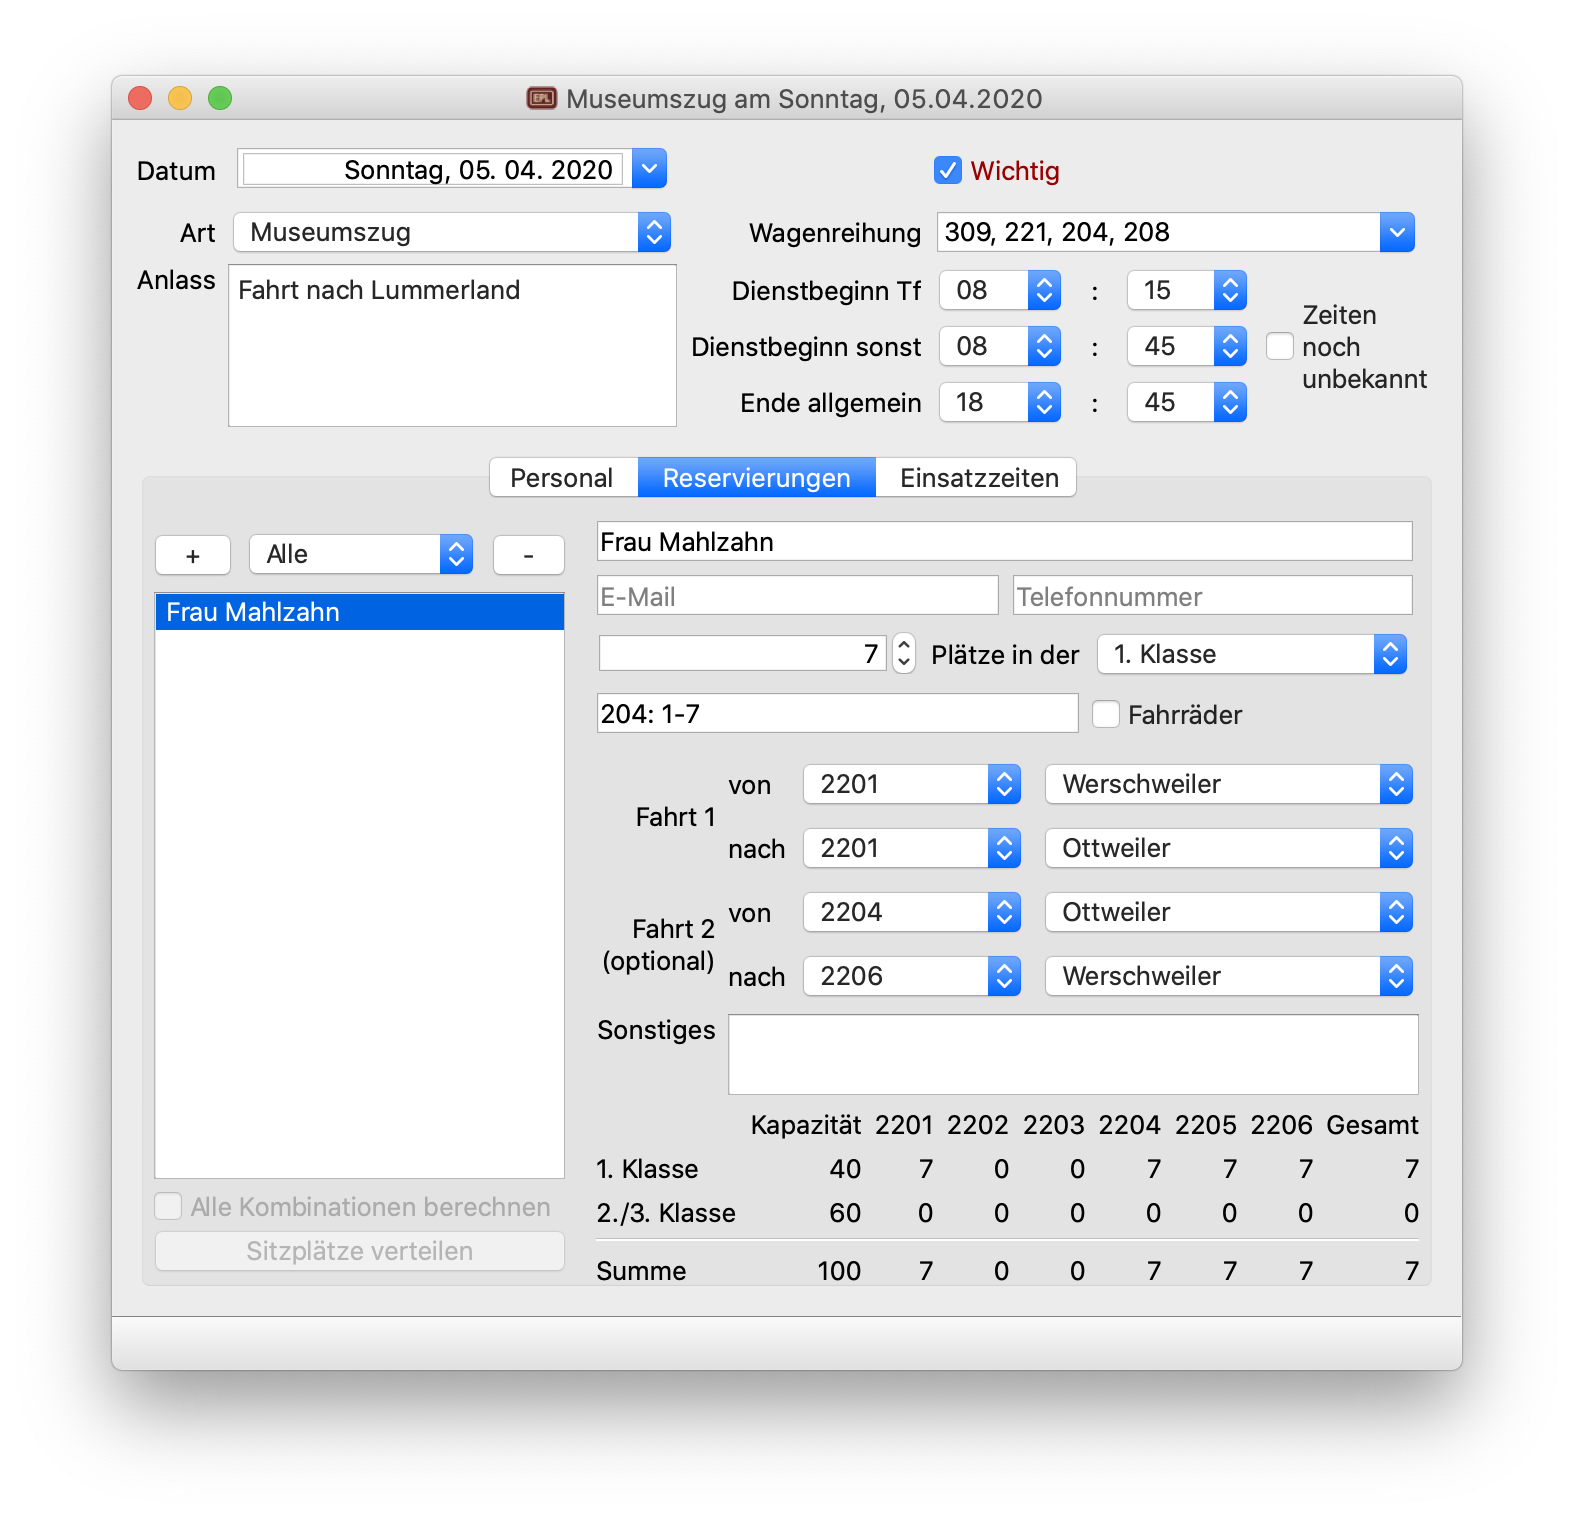
\includegraphics[width=\textwidth]{img/fahrtag_reservierungen}
	\caption{Das Fenster eines Fahrtags mit geöffnetem Tab für die Reservierungen.}
	\label{fig:einsatz:fahrtag:reservierungen}
\end{figure}
Im unteren Teil besteht die Möglichkeit die Reservierungen zu verwalten.
Eine Reservierung können Sie bearbeiten, indem Sie doppelt auf den Eintrag in der Liste klicken.
Sie wird dann in das Formular geladen. Dort können Sie die zugehörigen Information ändern.


Die Sitzplätze müssen in folgendem Format angegeben werden:
Zuerst der Wagen und dann die Sitzplätze durch Kommata getrennt.
Aufeinanderfolgende Sitzplatznummern können Sie durch das Format Von-Bis schreiben (Beispiel: \texttt{208: 6-12}).
Wenn Sie Plätze in mehreren Wagen angeben möchten,
müssen Sie die Plätze durch einen Strichpunkt voneinander trennen
(Beispiel: \texttt{204: 1-40; 217: 1-30}).


Die Fahrtstrecke kann dabei in zwei nichtzusammenhängende Teilstrecken unterteilt werden.
Im Folgenden finden Sie mögliche Beispiele, wie Fahrtstrecken optimal eingegeben werden können:
\begin{itemize}
	\item Eine Gruppe fährt in Zug 2202 von Ottweiler nach Schwarzerden und danach direkt wieder mit Zug 2203 zurück nach Ottweiler.\\
	Eingeben als:
	\begin{verbatim}Strecke 1  (2202 SOTW-SSWN) (Ottweiler)
           (2203 SSWN-SOTW) (Ottweiler)
Strecke 2  (-)              (-)
           (-)              (-)
	\end{verbatim}
	\item
	Eine andere Gruppe hat die gleiche Fahrstrecke, will aber eine Wanderung von Schwarzerden aus unternehmen und erst mit Zug 2205 wieder nach Ottweiler.
	Möglichkeit 1:
	\begin{verbatim}Strecke 1  (2202 SOTW-SSWN) (Ottweiler)
           (-)              (Schwarzerden)
Strecke 2  (2205 SSWN-SOTW) (Schwarzerden)
           (-)              (Ottweiler)
	\end{verbatim}
	Möglichkeit 2:
	\begin{verbatim}Strecke 1  (2203 SOTW-SSWN) (Ottweiler)
           (2203 SOTW-SSWN) (Schwarzerden)
Strecke 2  (2205 SSWN-SOTW) (Schwarzerden)
           (2205 SSWN-SOTW) (Ottweiler)
	\end{verbatim}
	\item
	Eine dritte Gruppe fährt von Schwarzerden nach Ottweiler in Zug 2201 und dann mit Zug 2202 von Ottweiler nach Fürth.
	Dort steigen Sie aus und fahren mit Zug 2204 wieder zurück nach Schwarzerden:
	\begin{verbatim}
Strecke 1  (2201 SSWN-SOTW) (Schwarzerden)
           (2202 SOTW-SSWN) (Fürth)
Strecke 2  (2204 SOTW-SSWN) (Fürth)
           (-)              (Schwarzerden)
	\end{verbatim}
\end{itemize}


\paragraph{Auswertung der Reservierungen}
Im linken unteren Teil des Fensters wird angezeigt,
wie viele Sitzplätze in den einzelnen Zügen bereits reserviert sind.
Diese Auslastung ist jeweils noch nach der ausgewählten Klasse (1.\ oder 2./3.~Klasse) unterteilt.
Ebenso wird die Summe der reservierten Sitzplätze für den jeweiligen Fahrtag angegeben.
In diese Gesamtsumme geht jede Reservierung nur einmal ein,
unabhängig von der angegebenen Fahrstrecke bzw.\ auch wenn keine angegeben ist.


\paragraph{Automatische Sitzplatzverteilung}
Wenn Sie bei der Art des Fahrtags eine Nikolausfahrt ausgewählt haben, haben Sie die Möglichkeit die Sitzplätze automatisch durch einen Druck auf den Knopf \aktion{Sitzplätze verteilen} zu verteilen.
Der Vorgang dauert in der Regel wenige Sekunden.
Es kann aber auch unter Umständen mehrere Minuten dauern.
Warten Sie diese Zeit bitte ab!
Wir arbeiten ständig an einer Verbesserung des Algorithmus zur Verteilung der Sitzplätze.

\begin{hinweis}
  Aktivieren Sie das Feld \button{Alle Kombinationen berechnen} nur, wenn Sie wenige Reservierungen angegeben haben (maximal 5-7),
  denn durch diese Auswahl wird der Rechenaufwand erheblich vergrößert!
\end{hinweis}



\section{Weiteres Personal}
\begin{figure}[!h]
	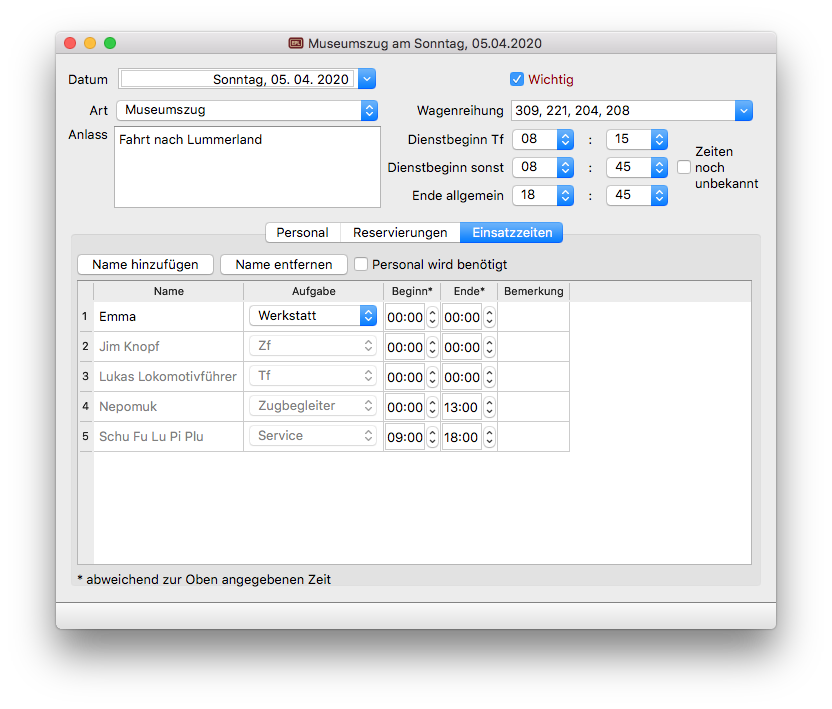
\includegraphics[width=\textwidth]{img/fahrtag_einsatzzeiten}
	\caption{Das Fenster eines Fahrtags mit geöffnetem Tab für das weitere Personal.}
	\label{fig:einsatz:fahrtag:einsatzzeiten}
\end{figure}

In der Tabelle von \cref{fig:einsatz:fahrtag:einsatzzeiten} erhalten Sie eine Übersicht über alle Personen,
die für diesen Fahrtag eingetragen wurden.
Zu jeder Person wird die Aufgabe angezeigt, die sie durchführt.
Die Arbeitszeit wird dann auf das entsprechende Konto angerechnet.
Es stehen die standardmäßigen Aufgaben (siehe \cref{glossar}) zum Einstellen zur Verfügung.

Personen die betriebliche oder regelmäßige Aufgaben haben und somit bereits im Reiter Personal in eine Liste eingetragen wurden, werden hier auch angezeigt.
Allerdings können nur die Einsatzzeiten dieser Personen verändert werden.
Diese Personen müssen in den entsprechenden Listen gelöscht werden.


Die Spalten "`Beginn"' und "`Ende"' dienen dazu, Uhrzeiten anzugeben, wenn Personen nicht für den kompletten angegebenen Zeitraum geholfen haben.
So kann man eine frühere Endzeit eingeben, wenn zum Beispiel eine Person nur am Vormittag half.
Die Zeit der Lokführer wird automatisch anhand von "`Beginn Tf"' berechnet,
sodass hier kein manueller Eintrag vorgenommen werden muss.



\section{Menü}
Im Menü Fahrtag gibt es die Möglichkeit die Einzelansicht des geöffneten Fahrtages zu exportieren.
Ebenso können die Reservierungen ausgegeben werden oder der Fahrtag nach einer Sicherheitsanfrage komplett gelöscht werden.



\section{Export der Reservierungen}
Beim Export von \enquote{normalen} Fahrtagen werden die Reservierungen mit ausgegeben.
Da bei Nikolausfahrten sehr viele Reservierungen vorliegen, werden Sie nicht bei der Einzelansicht des Fahrtags angegeben.
Stattdessen können Sie, wie bei allen anderen Fahrtagen auch,
die Funktion \aktion{Reservierungen drucken \dots} und \aktion{Reservierungen als PDF sichern \dots} im Menü \aktion{Fahrtag} nutzen.

Das exportierte Dokument enthält folgende Informationen zu einer Reservierung: Name, Anzahl Sitzplätze, Sitzplätze, Kommentare/Bemerkungen sowie den Zustieg, sofern er verschieden von Ottweiler ist.

Eine grafische Ansicht der Sitzplatzverteilung ist aktuell noch nicht möglich.
